\subsection{Relations between TS(M) and S(M)}

The canonical injection of M in TS(M) extends in a unique fashion to an algebra homomorphism of T(M) into TS(M) (III, p.~485, Prop. 1). By Prop. 2, (ii) of IV, p.~43, this homomorphism is the operator s of symmetrization. Since the algebra TS(M) is commutative there exists (III, p.~497) one and only one algebra homomorphism \(\varphi_{M}\) , called canonical, of the algebra S(M) into the algebra TS(M) such that the diagram

\pandocbounded{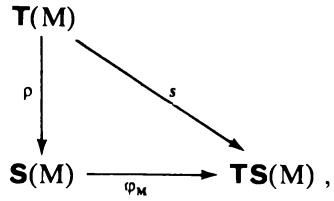
\includegraphics[keepaspectratio]{images/part001_42062a6f.jpg}}

where \(\rho\) denotes the canonical homomorphism of \(\mathbf{T}(\mathbf{M})\) onto \(\mathbf{S}(\mathbf{M})\) , is commutative. We have \(\varphi_{\mathbf{M}}(\mathbf{S}^{p}(\mathbf{M})) \subset \mathbf{T}\mathbf{S}^{p}(\mathbf{M})\) for all \(p \in N\) .

On the other hand, by composing the canonical injection i of TS(M) into T(M) with the canonical homomorphism \(\rho\) of T(M) onto S(M) we obtain a homomorphism \(\psi_{M}\) of graded A-modules, called canonical. The diagram

\pandocbounded{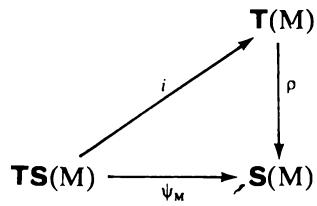
\includegraphics[keepaspectratio]{images/part001_38781a0a.jpg}}

is commutative.

If \(u: \mathbf{M} \to \mathbf{N}\) is a homomorphism of A-modules, then the diagram

\begin{enumerate}
\def\labelenumi{(\arabic{enumi})}
\setcounter{enumi}{12}
\tightlist
\item
\end{enumerate}

\pandocbounded{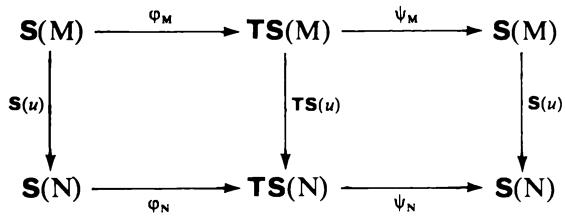
\includegraphics[keepaspectratio]{images/part001_026b2058.jpg}}

is commutative, as is easily verified.

If M is the direct sum of the modules \(M_{\lambda}\) , the diagram

\begin{enumerate}
\def\labelenumi{(\arabic{enumi})}
\setcounter{enumi}{13}
\tightlist
\item
\end{enumerate}

\pandocbounded{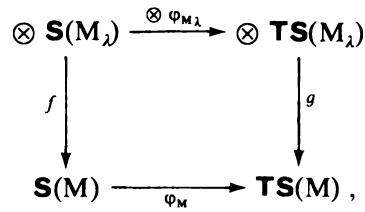
\includegraphics[keepaspectratio]{images/part001_9b5b14d2.jpg}}

where \(f\) and \(g\) are the canonical homomorphisms, is commutative. For \(g \circ \bigotimes_{\lambda} \varphi_{M_{\lambda}}\) and \(\varphi_{M} \circ f\) are algebra homomorphisms which coincide on \(M_{\lambda}\) for every \(\lambda\).

PROPOSITION 11. --- If M is free, then \(\varphi_{\mathbf{M}}\) is a morphism of graded bigebras.

Using the commutativity of the diagrams (13) and (14), we obtain the commutative diagram

\[
\begin{array}{l} \mathbf {S} (\mathrm{M}) \xrightarrow {\mathbf {S} (\Delta)} \mathbf {S} (\mathrm{M} \oplus \mathrm{M}) \xrightarrow {h} \mathbf {S} (\mathrm{M}) \otimes \mathbf {S} (\mathrm{M}) \\ \varphi_ {\mathrm{M}} \Bigg | _ {\downarrow} \quad \Bigg | _ {\varphi_ {\mathrm{M}} \oplus \mathrm{M}} \quad \Bigg | _ {\varphi_ {\mathrm{M}} \otimes \varphi_ {\mathrm{M}}} \\ \mathbf {T S} (\mathrm{M}) \xrightarrow [ \mathsf {T S} (\Delta) ]{} \mathbf {T S} (\mathrm{M} \oplus \mathrm{M}) \xrightarrow [ k ]{} \mathbf {T S} (\mathrm{M}) \cdot \otimes \mathbf {T S} (\mathrm{M}), \end{array}
\]

where \(\Delta\) is the diagonal homomorphism and h, k are canonical homomorphisms. The proposition follows from this.

PROPOSITION 12. --- (i) If \(u \in \mathbf{S}^n(\mathbf{M})\) , then \(\psi_{\mathbf{M}}(\varphi_{\mathbf{M}}(u)) = n!u\) .

\begin{enumerate}
\def\labelenumi{(\roman{enumi})}
\setcounter{enumi}{1}
\tightlist
\item
  If \(v \in \mathbf{T}\mathbf{S}^n(\mathbf{M})\) then \(\varphi_{\mathbf{M}}(\psi_{\mathbf{M}}(v)) = n!v\) .
\end{enumerate}

Let \(x_{1}, \ldots, x_{n} \in M\) and let u be the product \(x_{1} \ldots x_{n}\) calculated in \(\mathbf{S}(\mathbf{M})\) . Then \(\varphi_{\mathbf{M}}(u)\) is the product \(x_{1} \ldots x_{n}\) calculated in \(\mathbf{T}\mathbf{S}(\mathbf{M})\) , that is

\[
\sum_ {\sigma \in \mathfrak {S} _ {n}} x _ {\sigma (1)} \otimes \dots \otimes x _ {\sigma (n)}.
\]

Hence \(\psi_{\mathbf{M}}(\varphi_{\mathbf{M}}(u))\) equals \(\sum_{\sigma \in \mathfrak{S}_n}x_{\sigma (1)}\ldots x_{\sigma (n)}\) calculated in \(\mathbf{S}(\mathbf{M})\) , that is

\[
n! x _ {1} \dots x _ {n} = n! u.
\]

Let \(v = \sum_{i=1}^{p} x_1^i \otimes x_2^i \otimes \ldots \otimes x_n^i\) be an element of \(\mathbf{TS}^n(\mathbf{M})\) , where the \(x_j^i\) belong

to \(\mathbf{M}\) ; then \(\psi_{\mathbf{M}}(v)\) is equal to \(\sum_{i=1}^{p} x_1^i x_2^i \ldots x_n^i\) calculated in \(\mathbf{S}(\mathbf{M})\) , whence

\[
\varphi_ {\mathrm{M}} \big (\psi_ {\mathrm{M}} (v) \big) = \sum_ {i = 1} ^ {p} \mathbf {s} \big (x _ {1} ^ {i} \otimes x _ {2} ^ {i} \otimes \dots \otimes x _ {n} ^ {i} \big) = s (v) = n! v.
\]

COROLLARY 1. --- If A is a Q-algebra, then the canonical homomorphism of S(M) into TS(M) is an algebra isomorphism. If moreover M is free, then it is an isomorphism of graded bigebras.

COROLLARY 2. --- If A is a Q-algebra then the module \(\mathbf{TS}^n (\mathbf{M})\) is generated by the \(n\) -th powers of elements of \(\mathbf{M}\) in \(\mathbf{TS}(\mathbf{M})\) .

This follows from Cor. 1 and the corresponding property of \(\mathbf{S}(\mathbf{M})\) (III, p.~498).

